\chapter{Survey of Models}

On March 11, 2011 a magnitude 9.1 earthquake struck Japan, the epicenter just 76km from the eastern coast of the Tohoku region.  This caused a tsunami that collapsed a nearby nuclear reactor resulting in the Fukushima Daiichi Nuclear Disaster, a meltdown that resulted in 19,500 total deaths.  The reactor was built to withstand earthquakes up to 8.6 in magnitude.  The following example, inspired by (Silver, 2015)\cite{silver2015signal} illustrates a statistical model of annual earthquake frequencies of the greater Tohoku region.  Data was queried using the United States Geological Survey's ANSS Comprehensive Earthquake Catalog (ComCat).  The full analysis was conducted in R 4.2.2 and is detailed in the appendix of this thesis.  The purpose of this survey is to demonstrate the predictive capabilities of neural networks compared to a traditional model for this specific circumatance.  Three models are tested:
A Poisson regression model, a multi-layer perceptron network (MLP) with no regularization, and a multi-layer perceptron that employs Bayesian regularization in the manner described earlier (Bayesian Reglarized Neural Network, or BRNN). While no model surveyed will be used to extrapolate cases such as a magnitude 9.1, models could be apprehended for a future study and modified to accommodate such rare event predictions.

After pre-processing, the data was coerced into a table of earthquake sizes (measured by Richter magnitude rounded to one decimal place) and the average annual frequency \textit{at or above} each size in the greater Tohoku area over the 46-year span from 1965 up to the Great Quake of March 11, 2011. 
%Despite not being a full year, earthquakes recorded from January 1 to March 11, 2011 were still included to generate an overall average.  It was determined \textit{a-priori} that the most information was needed to determine precise annual frequencies leading up to the event.
The following plot was generated to display the data. There are 31 data points within the magnitude interval $[4.5,7.7]$.  Data was split 80/20 for training and testing respectively.  The surveyed models will be used to generate predictions of the \textit{expected annual frequency of each size earthquake}.  These models are evaluated based on the predictive accuracy on the 20\% held-out test set.  A mode with a smaller test error (calculated as the mean of the square differences between predictions and test data points) supposes a preferable model.

\begin{figure}[H]
    \center
    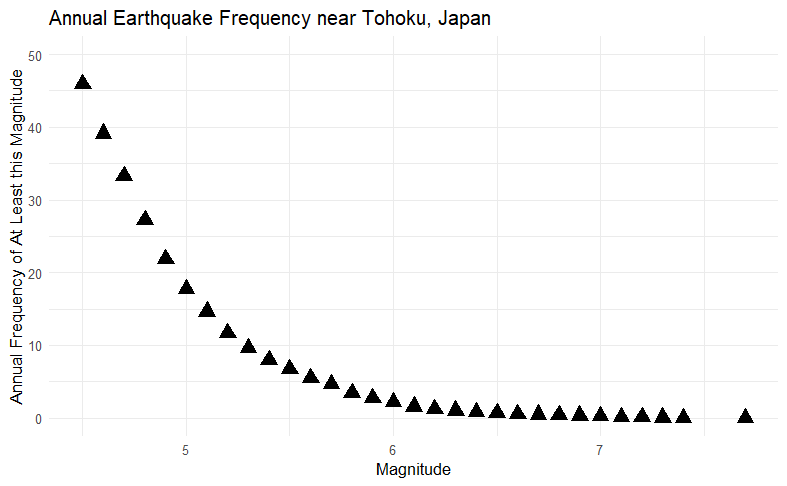
\includegraphics[width=0.75\linewidth]{Figures/tohoku_standardscale.png}
   % \vspace{-10pt}
    \caption{\footnotesize{Annual Tohoku earthquake frequencies of magnitude 4.5 and above.}}
    \label{tohoku_unfit}
\end{figure}


%---Pathway to earthquakes_lm_example file---
\subfile{earthquakes_lm_example}

%---Pathway to earthquakes_mlp file---
\subfile{earthquakes_mlp}

%---Pathway to earthquakes_brnn file---
\subfile{earthquakes_brnn}